\subsection{Эйлеровы циклы и пути}

\begin{defn}
    Эйлеров путь: путь без повторяющихся ребер, проходящий по всем ребрам графа.
\end{defn}

\begin{defn}
    Эйлеров путь, возвращающийся в исходную вершину: эйлеров цикл.
\end{defn}

\begin{theorem}~
    
    Связный  граф содержит эйлеров цикл $\iff$ все вершины в нем имеют четную степень.

    Связный граф содержит эйлеров путь $\iff$ он содержит две или ни одной вершины нечетной степени.

\end{theorem}

\begin{proof}
    
    "$\Rightarrow$":

    Очевидно: эйлеров путь, проходя каждую промежуточную вершину, использует два инцидентных ей ребра; следовательно, степени всех вершин, кроме начала и конца, четны. Аналогично для цикла.

    "$\Leftarrow$":

    Индукцией по количеству ребер сразу двух утверждений: предположим, что верно и для пути, и для цикла для графов с не более чем $n$ ребрами. Докажем, что верно для пути в графе с $(n + 1)$ ребром.

    Рассмотрим путь между двумя вершинами нечетной степени. Удалим его.

    Граф, возможно, распадется на компоненты связности, в каждой из которых степени всех вершин будут четными.

    Следовательно, в них по индукционному предположению будут существовать эйлеровы циклы.

    Будем двигаться в исходном графе по удаленному пути.

    Каждый раз, встречая вершину из очередной не обойденной компоненты, будем обходить ее по эйлерову циклу этой компоненты и продолжать движение по пути.

    Для цикла аналогично.

\end{proof}

\subsubsection*{Ориентированные графы}

\begin{theorem}~

    Сильно связный ориентированный граф содержит эйлеров цикл $\iff$ каждая его вершина имеет равные степень захода и степень исхода.

    Сильно связный ориентированный граф содержит эйлеров путь $\iff$ все его вершины, кроме возможно двух, имеют равные степень захода и степень исхода.

    Из двух особых вершин одна имеет степень исхода на единицу большую, чем степень захода, а другая --- степень захода на единицу большую, чем степень исхода.
\end{theorem}

\begin{proof}
    Аналогично доказательству теоремы для неориентированных графов.
\end{proof}

\subsubsection*{Граф де Брейна}

Граф порядка $n$ для $k$-символьного алфавита $\sum$:

\begin{itemize}
    \item множество вершин $V = \sum^n$.
    
    \item $k$ исходящих дуг у каждой вершины $w_1 \ldots w_n \in \sum^n$:
    
    для всех $b \in \sum$ дуга из $w_1 \ldots w_n$ в $w_2 \ldots w_n b$.
\end{itemize}

Для $n = 3,~k = 2$:

\begin{center}
    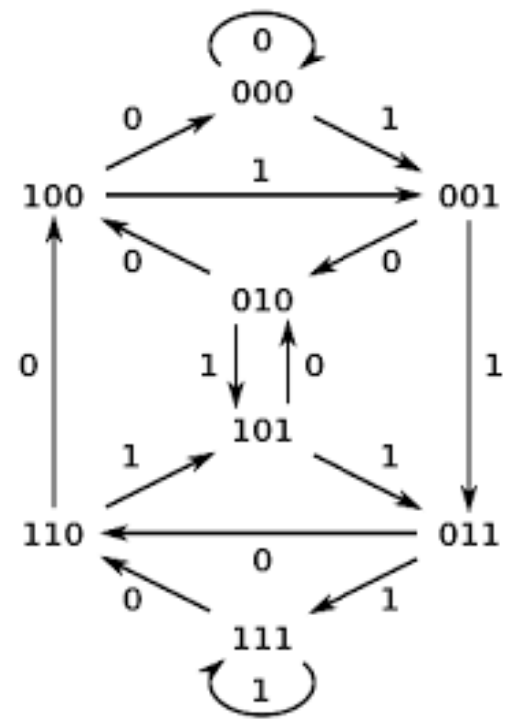
\includegraphics[width=0.25\textwidth]{par19brujin.png}
\end{center}

\begin{theorem}
    В графе де Брейна существует эйлеров цикл.

    Существует строка длины $k^{n+1} + n$, содержащая все подстроки длины $n + 1$.
\end{theorem}

\begin{proof}
    В каждой вершине $wb~(w \in \sum^{n - 1},~b \in \sum)$ ровно $k$ входящих дуг, идущих из всех вершин вида $aw$, для $a \in \sum$. Поэтому эйлеров цикл есть.

    Искомая строка строится так:

    \begin{itemize}
        \item сперва записывается произвольная $n$-символьная строка $w^0$,
        
        \item затем, начиная с вершины $w^0$, проходится весь эйлеров цикл
        
        \item при этом другие символы, соответствующие посещаемым дугам, приписываются к строке.
        
    \end{itemize}

    При прохождении дуги $b$ из вершины $aw$ в вершину $wb$ последние $n + 1$ символов строки равны $awb$, и все подстроки так обходятся.    
\end{proof}